\documentclass[a4paper,11pt]{kth-mag}
\usepackage[T1]{fontenc}
\usepackage{textcomp}
\usepackage{lmodern}
\usepackage[latin1]{inputenc}
\usepackage[swedish,english]{babel}
\usepackage{modifications}
\usepackage[acronym]{glossaries}
\usepackage{hyperref}
\usepackage{graphicx}
\usepackage{nameref}

\newcommand*{\fullref}[1]{\hyperref[{#1}]{\autoref*{#1} \nameref*{#1}}} % One single link

\makeglossaries

% Epigraph
%\epigraphfontsize{\small\itshape}
\renewcommand{\epigraphrule}{0pt}
\renewcommand{\epigraphflush}{flushright}
%\renewcommand{\textflush}{center}
\setlength{\epigraphwidth}{.7\textwidth}

% Glossary
\newglossaryentry{xpg}{name={XP},
    description={Extreme Programming (XP) is an agile development methodology where the developers usually works in pairs}}
\newglossaryentry{rpi}{name={runaway process inflation}, description={Runaway inflation is a very rapid inflation (decrease of money value). Runaway process inflation is a term sometimes used within agile development to describe rapidly growing development processes}}
\newglossaryentry{td}{name={technical dept}, description={Technical dept (also called design dept or code dept), is a metaphor primarily used in software development referring to the consequences of poor system design. The dept builds up as you for example introduce bugs and so called spaghetti code that has to be fixed in the future, as in repaying your dept}}

% Acronyms
\newglossaryentry{xp}{type=\acronymtype, name={XP}, description={Extreme Programming}, first={Extreme
Programming (XP)\glsadd{xpg}}, see=[Glossary:]{xpg}}



\title{Agile Development in a Solo Environment}

\subtitle{Duis autem vel eum iruire dolor in hendrerit in
          vulputate velit esse molestie consequat, vel illum
          dolore eu feugiat null}
\foreigntitle{Lorem ipsum dolor sit amet, sed diam nonummy nibh eui
              mod tincidunt ut laoreet dol}
\author{Mathias Lindblom}
\date{June 2015}
\blurb{Master's Thesis at KTH Royal Institute of Technology\\Computer Science and Communication (CSC)\\Supervisor: Sten Andersson\\Examiner: Olle B�lter}
 \trita{}
\begin{document}
\frontmatter
\pagestyle{empty}
\removepagenumbers
\maketitle
\selectlanguage{english}
\begin{abstract}
  This is a skeleton for KTH theses. More documentation
  regarding the KTH thesis class file can be found in
  the package documentation.

Lorem ipsum dolor sit amet, consectetuer adipiscing elit. Mauris
purus. Fusce tempor. Nulla facilisi. Sed at turpis. Phasellus eu
ipsum. Nam porttitor laoreet nulla. Phasellus massa massa, auctor
rutrum, vehicula ut, porttitor a, massa. Pellentesque fringilla. Duis
nibh risus, venenatis ac, tempor sed, vestibulum at, tellus. Class
aptent taciti sociosqu ad litora torquent per conubia nostra, per
inceptos hymenaeos.
\end{abstract}
\clearpage
\begin{foreignabstract}{swedish}
  Denna fil ger ett avhandlingsskelett.
  Mer information om \LaTeX-mallen finns i
  dokumentationen till paketet.

Lorem ipsum dolor sit amet, consectetuer adipiscing elit. Mauris
purus. Fusce tempor. Nulla facilisi. Sed at turpis. Phasellus eu
ipsum. Nam porttitor laoreet nulla. Phasellus massa massa, auctor
rutrum, vehicula ut, porttitor a, massa. Pellentesque fringilla. Duis
nibh risus, venenatis ac, tempor sed, vestibulum at, tellus. Class
aptent taciti sociosqu ad litora torquent per conubia nostra, per
inceptos hymenaeos.
\end{foreignabstract}
\clearpage
\tableofcontents*
\mainmatter
\pagestyle{newchap}

\chapter{Introduction}
This chapter will initially go through the problem statement and goals of the report. It will also show the motivation and estimated value of the entire report. The last section will outline the structure of the rest of the report.

Agile development is something

\section{Problem Statement}
\noindent
\newline
The hypothesis being tested is:

\begin{itemize}
\item There are agile development methods and strategies suitable for small development groups consisting of as little as one person.
\end{itemize}

The question regarding how this hypothesis can be tested is quite hard. It is obvious that agile development strategies can be used in small groups or when working solo, hence the word \emph{suitable}. However the word is ambiguous but it also should be given vagueness of the evaluation methods. It is important to realize that what is being evaluated is very complicated for explained reasons and to test the hypothesis one would have to conduct a rather large study, preferably both quantitative and qualitative, over a long period of time. In reality, the results of this thesis will give indications rather than answers and could be used in a research of larger scope that justifies the topic.

\section{Goals}
The main goal of the thesis is as follows:

\begin{itemize}
\item Produce an agile development plan or agile strategies suitable for a single developer up to small teams consisting of only a few people.
\end{itemize}
\noindent
Secondary goals:

\begin{itemize}
\item Theoretical comparison of popular agile development methods such as for example Scrum, \gls{xp}, Kanban etc. 
\item Overall clarification of agile terms and thinking/reasoning. For example differentiate Agile from Lean.
\end{itemize}

\section{Motivation \& Value}
Agile software development can be seen as a trend in today's computer industry and the actual concept of the method changes every year, which is quite appropriate given what the methodology advocates. The method mainly targets advanced systems and encourage continuous improvement and rapid changes to new customer demands. The development process revolves around having collaboration between self-organizing and cross-functional teams with focus on communication together with a iterative development process. However the information available regarding how-to practically establish an agile development process in small companies with small projects is limited. The available literature usually give hints on where to start but focuses heavily on the full blown methods and leaves it up to the reader to decide what is practically possible for their limited sized development group or company.

\section{Thesis Report Outline}


\chapter{Agile Development}

Most developers have experienced the nightmare of working on a project and slowly witness the increasing number of bugs, errors and time when adding new functionality. In order to combat this disheartening scenario, developers created constraints and routines around their activity, forming a development process based on prior mistakes. However big development projects can be complex and even though experienced based constraints helps, at some point the problems reappear. The solution for this was to keep adding more constraints and routines. So the development process grows and grows and until the process itself has become so cumbersome and advanced that it creates the problems it was designed to prevent, which is to avoid \gls{td} and increase efficiency\cite{key1}. This so called \gls{rpi} was common among big companies around the millennium shift and at the time it was a growing negative trend \cite{key1}. This issue, that software teams around the world experienced, was observed by a few industry experts calling themselves the Agile Alliance who sought to fight it \cite{key1}. The ideas that make up agile development were not new at the time but it was the Agile Alliance that formulated the underlying concepts that make up agile development. Read more about this at \fullref{sec:manifesto}.

\section{Abstraction \& Components}
It is common that agile development is directly compared to the waterfall model which is strange given how they situate on different abstraction levels. The waterfall model is a software development methodology just like Scrum. Agile development on the other hand is not a followable methodology by itself. It is more of an ideology or perhaps a collection of methodologies. So how is it even possible to compare the two of them? The answer is that people are comparing the waterfall model to some popular agile methodology like Scrum or just some common practices like sprints and pair programming, indirectly claiming that these elements represent agile development as a whole. This leads to confusion and unfair comparisons. So before continuing reading about agile development it is a good idea to get a better understanding of the components that make up agile development. 

In Figure \ref{fig:agile_abstraction}, agile development have been dividid into 4 different abstraction levels. First we have the ideology that consist of the core ideas such as the agile manifesto and principles. Secondly we have the methodologies and strategies that try to fulfill all or some of the agile principles or mentalities. The third abstraction are the practices that make up the methodologies. These practices can be similar to the agile principles but they are more practically applicable and at a much lower abstraction level. Each practice tries to satisfy one or several of the agile principles. Lastly, at the forth abstraction level, we have the actual tools that are needed to make the practices a reality. These tools can be very simple such as a physical room for meeting practices or more advanced such as xUnit for test-driven development.

\begin{figure}[h]
  
  \centering
    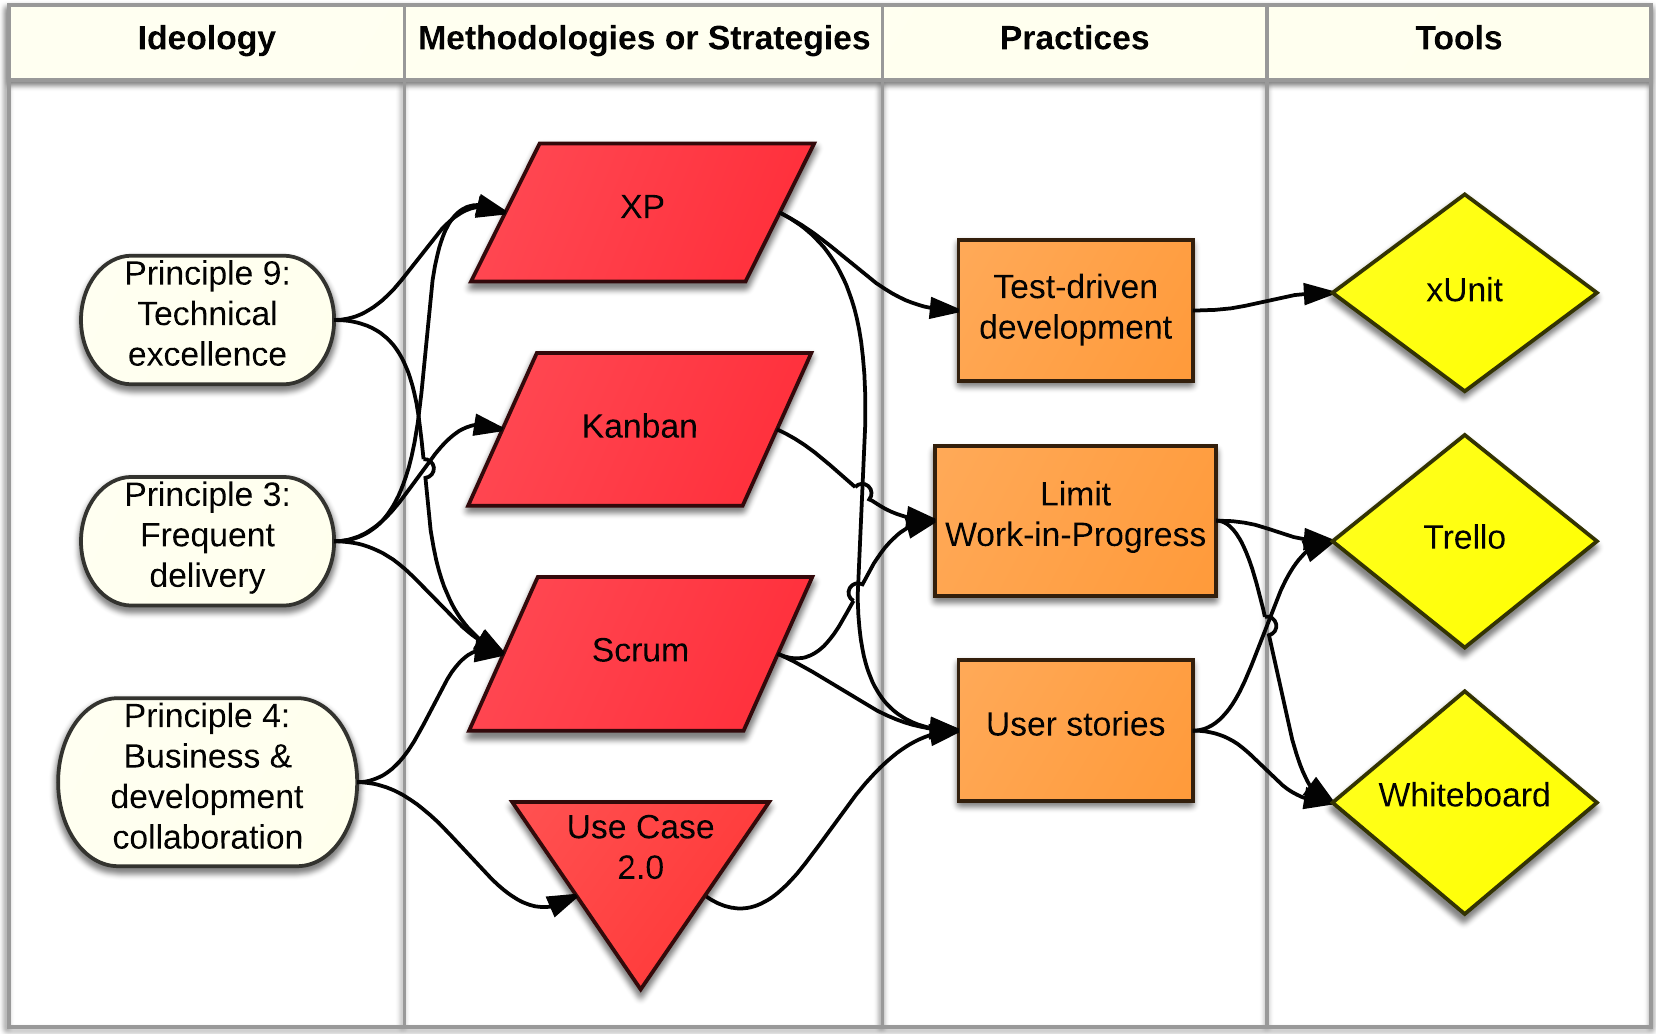
\includegraphics[width=1.0\textwidth]{img/agile_development_abstraction.png}
    \caption{Agile development divided in four different abstraction levels and how the example elements within them correlate to each other.}
    \label{fig:agile_abstraction}
\end{figure}




\section{The Agile Manifesto}
\label{sec:manifesto}
The Agile Alliance is an organization formed by a group of computer industry experts in 2001. They decided to come together in order to form general development values in order to improve the software development process for companies around the world \cite{key1} \cite{key2}. The result was The Agile Manifesto that states the following:

\begin{itemize}
\item \textbf{Individuals and interactions} over processes and tools.
\item \textbf{Working software} over comprehensive documentation.
\item \textbf{Customer collaboration} over contract negotiation.
\item \textbf{Responding to change} over following a plan.
\end{itemize}

The group that wrote The Agile Manifesto consisted of the following people: Kent Beck, Mike Beedle, Arie van Bennekum, Alistair Cockburn, Ward Cunningham, Martin Fowler, James Grenning, Jim Highsmith, Andrew Hunt, Ron Jeffries, Jon Kern, Brian Marick, Robert C. Martin, Steve Mellor, Ken Stewier, Jeff Sutherland, Dave Thomas \cite{key1} \cite{key2}.

The following four subsections will give a short explanation for each of the statements of The Agile Manifesto that stands as the highest abstraction or the core that is agile development.

\subsection{Individuals and Interactions over Processes and Tools}

\epigraph{Process and technology are a second-order effect on the outcome of a project. The first-order effect is the people. \cite{key1}}{\textsc{Alistair Cockburn}}
\noindent
Within football most agree that a football team of average players that communicate well can beat a team of egoistic superstars. The same goes for software development (and probably many more things) where a team of average programmers working together outperforms a team of expert programmers that fail to communicate. At least according to the thinking and reasoning of agile development \cite{key1}.

Processes and tools are of course important as well but not as important. After all, agile development methodologies are processes that usually requires tools. Team managers have a habit of setting up the development environment and then assigning a team, assuming that the team will work well since they have the tools they need \cite{key1}. However this is focus put at the wrong end of order. Tools and processes can rarely repair a team that doesn't play ball but a functioning team is usually capable of configuring their own environment \cite{key1}.

\subsection{Working Software over Comprehensive Documentation}

\epigraph{The program is the specification and documentation. \cite{key3}}{\textsc{Douglas Crockford}}

\noindent
This might not be that much of a shocker, that functioning software is more important than documentation. The keyword here is \emph{comprehensive} since it is common that teams get hung up on the quest of having close to 100 percent coverage on documentation \cite{key1}. The problem with this is that it takes a lot of time and effort to always keep in sync with the code and as soon as you lose the sync, the documentation begins telling lies. Instead of having every technical part of a program described in a thick book it is usually preferred, both for the reader and the writer, to have a short rational and structured document that explains the software at a high abstraction. When a new member of a team needs more technical information they will get it when working closely and interacting with their team members and the actual software \cite{key1}.

A common misconception is that code is for the computer and documentation for the human to understand the code \cite{key4}. Instead of translating the code into human language, why can't we write code so that humans can understand it in the first place? We already do it by naming things like classes and methods with understandable names, but is usually ends there. We make it \emph{good enough}. If we instead focused more on the quality and logic of the code, a comprehensive documentation should not be needed at all. 

\subsection{Customer Collaboration over Contract Negotiation}
Many have tried to create strict contracts with fixed specifications, deadlines and prices for software development. Many have failed \cite{key3}. You simply can't treat software as a commodity expecting everything to be known before hand. Trying to do so can lead to all sorts of avoidable problems like poor quality or even complete failure. It is not only the complexity of programming that is the issue but also how fast our technical world changes over short time periods. This is one of the core problems that agile development tries to avoid. By having a tight collaboration with the customer, the specifications, deadlines and prices don't need to be as strict. Instead of having a contract specifying the exact requirements of the entire project it should instead address how the collaboration between customer and developers should be conducted \cite{key3}. This leads to a more dynamic development approach where technical problems can be addressed directly. More over, needed changes don't risk breaking the contract.

\subsection{Responding to Change over Following a Plan}	
Some of the reasons for this priority is stated in the previous  section regarding customer collaboration. Customers have a habit of not knowing what they really want or change their requirements after seeing some of the functionality coming to life \cite{key3}. Also like stated in the previous section about collaboration, the IT world we live in rapidly changes and so can the requirements of a software project. It is nice and tempting to have the full project planned in some advanced planning software with every functionality written. However as the development team and customer moves forward the plan is bound to change. Some functionality will no longer be deemed necessary and previously unthought of functionality might be added. Some parts of the strict plan might then have been a waste of time and more importantly, the strict plan might hinder these kind of positive changes that are needed or are advantageous to the project. 

By having a more abstract and lose plan with details only for the near future, for example a couple of weeks, you get a planning more susceptible to change \cite{key3}. That detailed plan can be strict but since it is only for a short time period the risks of having unneeded functionality or hindering change is limited. The further away in time we look the weaker the plan should be since we want flexibility to changes and the likelihood of changing requirements grows as the timeline increases.

\section{The Agile Principles}
Using the values stated by The Agile Manifesto, 12 principles were created that act as the characteristics for agile practices \cite{key1}. You can interpret these principles as the next abstraction step from The Agile Manifesto where you get a clearer explanation of what agile development is. These are the principles:

\begin{enumerate}
\item Our highest priority is to satisfy the customer through early and continuous delivery of valuable software.
\item Welcome changing requirements, even late in development. Agile processes harness change for the customer's competitive advantage.
\item Deliver working software frequently, from a couple of weeks to a couple of months, with a preference to the shorter timescale.
\item Business people and developers must work together daily throughout the project.
\item Build projects around motivated individuals. Give them the environment and support they need, and trust them to get the job done.
\item The most efficient and effective method of conveying information to and within a development team is face-to-face conversation.
\item Working software is the primary measure of progress.
\item Agile processes promote sustainable development. The sponsors, developers, and users should be able to maintain a constant pace indefinitely.
\item Continuous attention to technical excellence and good design enhances agility.
\item Simplicity--the art of maximizing the amount of work not done--is essential.
\item The best architectures, requirements, and designs emerge from self-organizing teams.
\item At regular intervals, the team reflects on how to become more effective, then tunes and adjusts its behavior accordingly.
\end{enumerate}





\section{Misconceptions}

\section{Agile vs Waterfall}

\section{Agile vs Lean}

\chapter{Agile Methodologies}
Up to this point the ideology, that is agile development, have been described. In this chapter the more common methodologies that try to adapt these ideas and mentalities will be described. In other words, the methodologies described here will contain more practically applicable agile practices. What is important to note is that every agile methodology is subject to change. Most advocates of some agile methodology encourages changes in the methodology to suit your development team and/or company. This means that the descriptions of the methodologies can look slightly different, especially when they have been written years apart. Another reason can be that some methodologies or practices within a methodology can be very vague resulting in different interpretations. However this does not mean that some descriptions of the practices are wrong. The reason for the vagueness is that the founders of the methodologies want to encourage changes and alternative implementations. 

Each methodology described will have an introduction followed by subsections that describes the core practices for the methodology. 

\section{Scrum}
\subsection{Roles}
\subsubsection{Product Owner}
\subsubsection{Development Team}
\subsubsection{Scrum Master}
\subsection{Events}
\subsubsection{Sprint}
\subsubsection{Meetings}
\subsubsection{Extensions}
\subsection{Artifacts}
\subsubsection{Product backlog}
\subsubsection{Sprint backlog}
\subsubsection{Product Increment}
\subsubsection{Sprint Burndown chart}
\subsubsection{Release burndown chart}

\section{Dynamic Systems Development Method (DSDM)}

\section{Extreme Programming (XP)}
\gls{xp} 
\subsection{Fine-Scale Feedback}
\subsubsection{Pair Programming}
\subsubsection{Planning Game}
\subsubsection{Test-Driven Development}
\subsubsection{Whole Team} 
\subsection{Continuous Process}
\subsubsection{Continuous Integration)}
\subsubsection{Refactoring}
\subsubsection{Small Releases}
\subsection{Shared Understanding}
\subsubsection{Coding Standards}
\subsubsection{Collective Code Ownership}
\subsubsection{Simple Design}
\subsubsection{System Metaphor}
\subsection{Programmer Welfare}
\subsubsection{Sustainable Pace}



\section{Kanban}
\subsection{Visualize}
\subsection{Limit Work-in-Progress}
\subsection{Manage Flow}
\subsection{Make Process Policies Explicit}
\subsection{Implement Feedback Mechanisms}
\subsection{Improve Collaboratively \& Evolve Experimentally}


\chapter{Method}
The method is divided in two main parts. The first section describes the theoretical evaluation of agile methodologies. The second part describes the project that has been developed using a few selected agile strategies.

\section{Theoretical Evaluation of Methodologies}

\subsection{Agile Methodology Point System} 

\section{Practical Evaluation of Agile Project}

\subsection{Project Description}
The actual project, to be developed using agile strategies, is a private initiative from Per-Arne Forsberg who has 25 years of successful international experience and knowledge in managing technically skilled units, products and projects around the world at Ericsson. Having been involved and engaged in change management, using the latest Lean and Agile methodology.
The project is developing a dynamic, scalable and robust interactive tutoring framework prototype for pre-academic students. Assisting students today according to the ?old school? is social but also ineffective since it is usually one to one communication or one to a few in a geographical location (you have to meet at pre-determined location at pre-determined times, like classrooms). The long term goal is to assist in communication between students and teachers (tutors willing to help out with their knowledge from their preferred location) in Sweden and in turn combat the negative (knowledge) grade curve that can be seen around the country (according to international studies, PISA). In short the idea is to create a interactive website that can be used for many to many type of communication between students and teachers. An exact specification of the project does not exist in order to encourage the agile development process.

\subsection{Chosen Methodology and/or Strategy}


\chapter{Results}


\section{Theoretical}

\subsection{Point System}

\section{Practical}

\subsection{Project}

\subsection{Developer \& Product Owner Experience}


\chapter{Discussion}


\section{Result Critique}

\section{Conclusions}

\subsection{Developers Thoughts}

\section{Future Work} 


\printglossary[type=main]
\nopagebreak[4]
\printglossary[type=\acronymtype]


\appendix
\addappheadtotoc
\chapter{RDF}\label{appA}

\begin{figure}[ht]
\begin{center}
And here is a figure
\caption{\small{Several statements describing the same resource.}}\label{RDF_4}
\end{center}
\end{figure}

that we refer to here: \ref{RDF_4}

\begin{thebibliography}{56}

\bibitem{key1}
Martin C. Robert, Martin Micah,
\emph{Agile Principles, Patterns, and Practices in C\#}.
Prentice Hall, Massachusetts,
2nd edition,
2006.

\bibitem{key2}
\url{http://www.agilealliance.org}

\bibitem{key3}
\url{https://www.youtube.com/watch?v=t9YLtDJZtPY&t=175}

\bibitem{key4}
\url{http://www.literateprogramming.com/knuthweb.pdf}

\end{thebibliography}

\end{document}
